\chapter{Evaluation of the Fitting with the Segmentation of the FCN}
The EM-algorithm-like method of Egger et al \cite{egger_paper} uses a binary mask to determine whether a pixel is relevant for the fitting-process or not. We changed the method of Egger et al to not estimate a mask itself, but to use the segmentation of the FCN in each iteration.\\
\\
As the Morphable Model, we use the popular Basel Face Model of 2017 \cite{BFM2017} which was originally proposed in 1999 by Blanz and Vetter \cite{BlanzVetter}. This model is used by the fitting process, but also by the parametric face image generator of Kortylewski et al \cite{parametric} which outputs renderings of sample facial images, the ground truth parameters of the face, and provides a ground truth segmentation. These ground truth data gets compared to the parameters of the fit.\\
\\
The experiments in this chapter will only be explained with one specific type of occlusions (hands) so as not to overwhelm the reader. Of course, we repeated the experiments on other occlusions types such as microphones, glasses, random boxes, and without any occlusion. Please find these fits and the error-plots in the appendix [\Cref{appendix:otherDatasets}].

\section{Experimental Setup}

For the evaluation of the fitting, we generated faces with 50 shape parameters of the Basel Face Model, another 50 for the colour and 50 for the expression. We now render different faces with various occlusions, diverse rotations/poses, a random illumination and cover them with different occlusions.\\
\\
The aim of this chapter is to reconstruct the generated synthetic faces with the EM-like algorithm of Egger et al which originally estimates fitting parameters and a segmentation itself. But we manipulate the algorithm such that it skips the E-step and takes the segmentation of the FCN, the ground truth segmentation, or no mask in every iteration. To get acceptable results we fix the number of EM steps to 20. In each iteration, 1000 samples are drawn. We measure the fitting accuracy and speed in this experiment, without letting the fitting algorithm produce its own z-labels. The FCN is trained to cut hands, glasses, and microphones out of the picture. That's why in the following experiments we use these three classes of occlusions. With the mask of the FCN, the fitting should  also be much faster, because the time-consuming job of updating the z labels is eliminated. After every iteration, we get information about the pose, the probability of the current sample, and about the 3DMM parameters of the fit. We compare those to the ground truth information from the parametric face image generator. To calculate the error, RMSE (Root Mean Squared Error) is used.

\section{Evaluation on the Tailored Face}
In this setting, we use the 'face12' version of the Basel Face Model. In contrast to the original, it has no neck, no ears, and no hairline. In every iteration the errors of the parameters of the Basel Face Model, the rotations, the illumination, and the probability of the best of the 1000 samples are measured [\Cref{fig:chap3:plot_hands_setup1}]. The experiments are repeated 10 times with different faces.\\ 
\\
We see that in the three parameters (shape, colour, and expression) the quality of the fit with the FCN segmentation is very close to the one of the iterative approach of Egger et al. The differences in the Euler rotations (yaw, pitch, and roll) are negligible, since all errors move in a very small order. The plot named 'EnvironmentMap' [\Cref{fig:chap3:plot_hands_setup1}], shows the deviation of the illumination parameters. These parameters simulate different light sources around the face.\\
\\
Since the evaluation data consists of occluded synthetic-facial images where the exact position and shape of the face is known, the masks used consist of the ground truth segmentation, the segmentation of the FCN, the occlusion-aware segmentation proposed by Egger et al \cite{egger_paper}, and a dummy mask where each pixel is segmented as face [\Cref{fig:chap3:zlabelsandfits}].

\pagebreak

\begin{figure}[H]
	\centering
	\subbottom[original facial image]{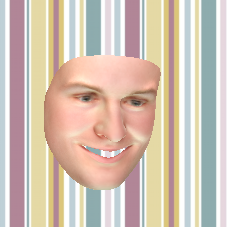
\includegraphics[width=.35\textwidth]{Figures/chap3/hands_setting1_original_test6.png}\label{fig:chap3:hands_original}}\qquad
	\subbottom[facial image with occlusion]{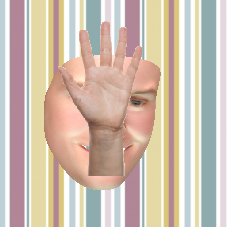
\includegraphics[width=.35\textwidth]{Figures/chap3/hands_setting1_occluded_test6.png}\label{fig:chap3:hands_occluded}}
	\caption{These pictures show the faces that should be modeled with different masks. We fit with the method Egger et al \cite{egger_paper} from \Cref{fig:chap3:hands_occluded} a face as similar as possible to the face in \Cref{fig:chap3:hands_original}.}
	\label{fig:chap3:hands_PARAMETRIC}
\end{figure}


\begin{figure}[H]
\newcolumntype{C}{>{\centering\arraybackslash} m{2.9cm} }  %# New column type
	\begin{tabular}{m{1.3cm}|SC|SC|SC|SC}
		& \parbox{2cm}{ground truth mask}& Egger & FCN & no mask\\ \hline
		z-labels & \subfloat{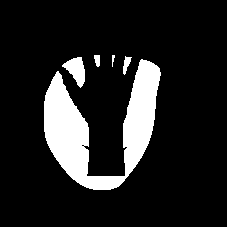
\includegraphics[width=0.16\textwidth]{Figures/chap3/hands_test6_mask_GROTRU.png}} &
		\subfloat{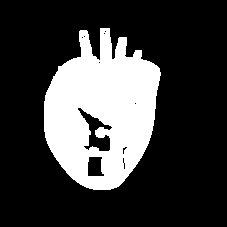
\includegraphics[width=0.16\textwidth]{Figures/chap3/hands_test6_mask_EGGER.png}} &
		\subfloat{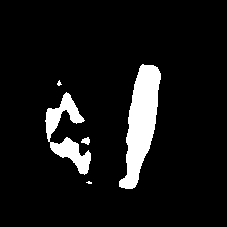
\includegraphics[width=0.16\textwidth]{Figures/chap3/hands_test6_mask_FCN.png}} & \\ \hline
		fits & \subfloat{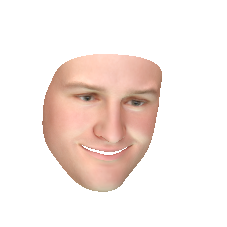
\includegraphics[width=0.16\textwidth]{Figures/chap3/hands_test6_fit_GROTRU.png}} &
		\subfloat{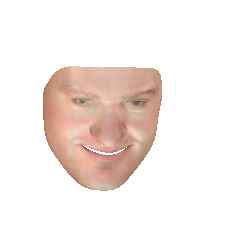
\includegraphics[width=0.16\textwidth]{Figures/chap3/hands_test6_fit_EGGER.png}} &
		\subfloat{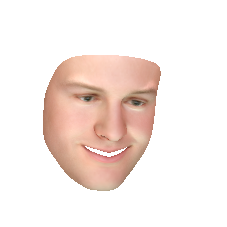
\includegraphics[width=0.16\textwidth]{Figures/chap3/hands_test6_fit_FCN.png}} &
		\subfloat{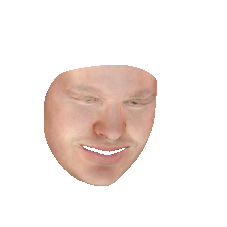
\includegraphics[width=0.16\textwidth]{Figures/chap3/hands_test6_fit_DUMMY.png}} \\
	\end{tabular}
	\caption{In the top row are the different segmentations we use for our experiments. The segmentation of Egger et al (second image from left) was calculated iteratively. Only the final mask is given. In the second row are the particular fits, when the above z-labels are used as mask. You can see that the fits without any mask (no mask) and the fits with the mask according to Egger et al (Egger) are far away from the true face depicted in [Figure \ref{fig:chap3:hands_original}]. However, the fits with ground truth mask of the parametric face image generator (ground truth mask) and the one with the FCN-Segmentation (FCN) come very close to the original.}
	\label{fig:chap3:zlabelsandfits}
\end{figure}

\begin{figure}[H]
	\centering
	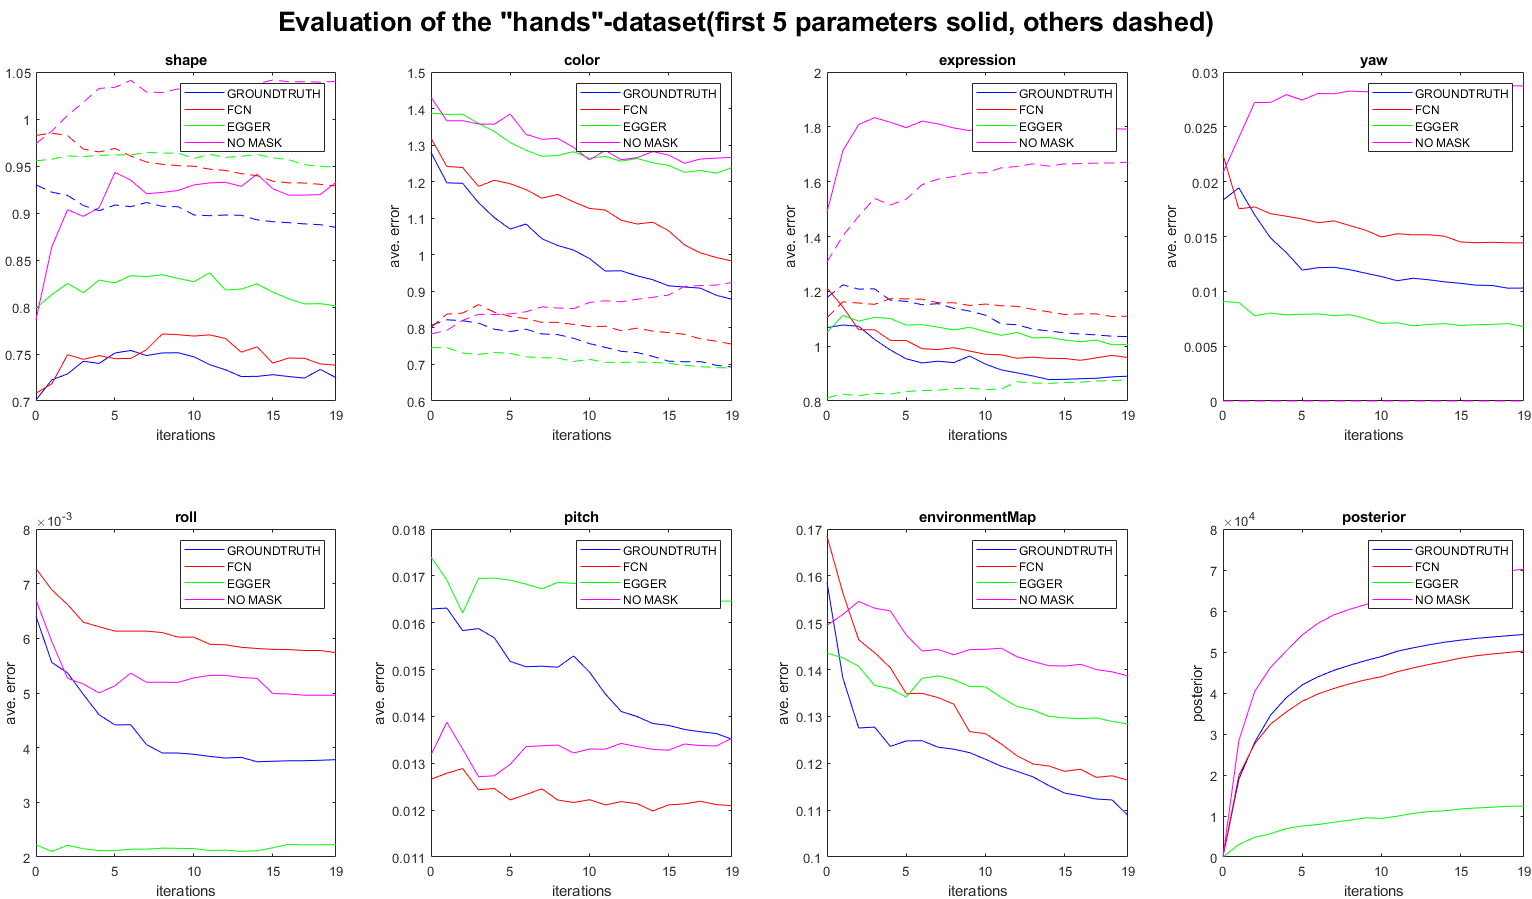
\includegraphics[angle=90,width=.55\textheight]{Figures/chap3/plot_hands_setting1.png}
	\caption{The first three plots show the errors of the first 50 shape, color and expression parameters of the Basel Face Model (in standard deviations). The next three show the errors of the Euler angles in radian. The 'EnvironmentMap'-plot shows the illumination chosen by all methods. In the last plot, we see the unnormalized posterior-probability, with which an Metropolis-Hastings sample was accepted.}
	\label{fig:chap3:plot_hands_setup1}
\end{figure}

\FloatBarrier

\section{Evaluation on the Original Face}
\label{sec:Oversegmentation}
In most cases, the fit with the FCN mask is not as different from the fit with the Egger mask itself as shown in [Figure \ref{fig:chap3:zlabelsandfits}]. However, we find that Egger's method tends to segment all skin pixels, whether they belong to the face or not. That's why in a next step we create faces with the 'bfm' version of the Basel Face Model. These faces are not tailored and include ears, hairline, and neck. We expect the segmentation of Egger et al to segment these areas too.

\begin{figure}[H]
	\centering
	\subbottom[original facial image]{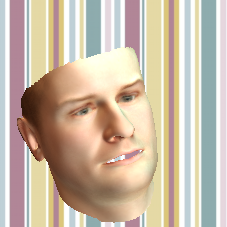
\includegraphics[width=.4\textwidth]{Figures/chap3/hands_setting2_test0_original.png}\label{fig:chap3:hands_setting2_original}}\qquad
	\subbottom[facial image with occlusion]{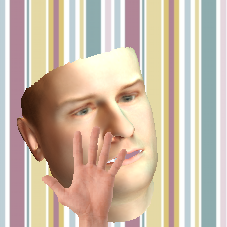
\includegraphics[width=.4\textwidth]{Figures/chap3/hands_setting2_test0.png}\label{fig:chap3:hands_setting2_occluded}}
	\caption{These pictures are different from the ones in Figure \ref{fig:chap3:hands_PARAMETRIC} because we now use the 'bfm' version of the Basel Face Model which contains more skin pixels than the 'face12' version. The fitting algorithm takes \ref{fig:chap3:hands_setting2_occluded} as input and tries to approximate \ref{fig:chap3:hands_setting2_original}.}
	\label{fig:chap3:hands_setting2_PARAMETRIC}
\end{figure}

\begin{figure}[H]
	\newcolumntype{C}{>{\centering\arraybackslash} m{2.4cm} }  %# New column type
	\begin{tabular}{m{1.3cm}|SC|SC|SC|SC}
		& \parbox{2cm}{ground truth mask}& Egger & FCN & no mask\\ \hline
		z-labels & \subfloat{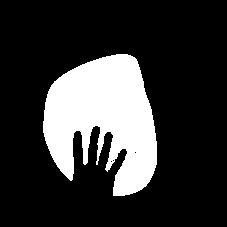
\includegraphics[width=0.16\textwidth]{Figures/chap3/hands_test0_mask_GROTRU_.png}} &
		\subfloat{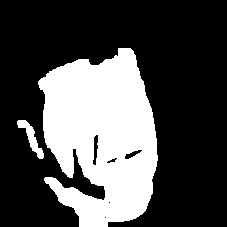
\includegraphics[width=0.15\textwidth]{Figures/chap3/hands_test0_mask_EGGER_.png}} &
		\subfloat{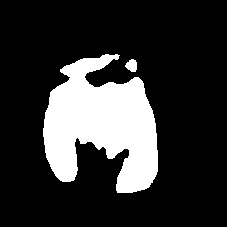
\includegraphics[width=0.15\textwidth]{Figures/chap3/hands_test0_mask_FCN_.png}} & \\ \hline
		fits & \subfloat{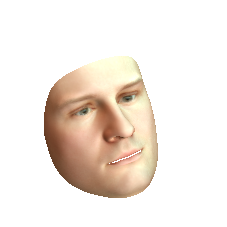
\includegraphics[width=0.15\textwidth]{Figures/chap3/hands_test0_fit_GROTRU.png}} &
		\subfloat{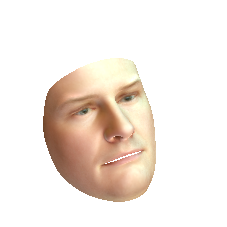
\includegraphics[width=0.15\textwidth]{Figures/chap3/hands_test0_fit_EGGER.png}} &
		\subfloat{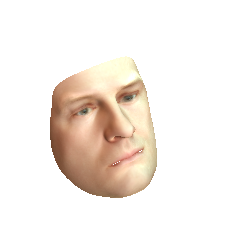
\includegraphics[width=0.15\textwidth]{Figures/chap3/hands_test0_fit_FCN.png}} &
		\subfloat{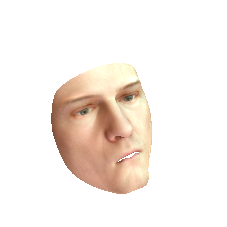
\includegraphics[width=0.15\textwidth]{Figures/chap3/hands_test0_fit_DUMMY.png}} \\
	\end{tabular}
	\caption{In the top row, the different mask can be seen. The segmentation of Egger is updated in every iteration of the fitting process and only the mask in the last step is given. It is obvious that Egger oversegments and labels too much as face. The bottom row shows the fits with the masks above.}
	\label{fig:chap3:zlabelsandfits_setting2}
\end{figure}

\begin{figure}[H]
	\centering
	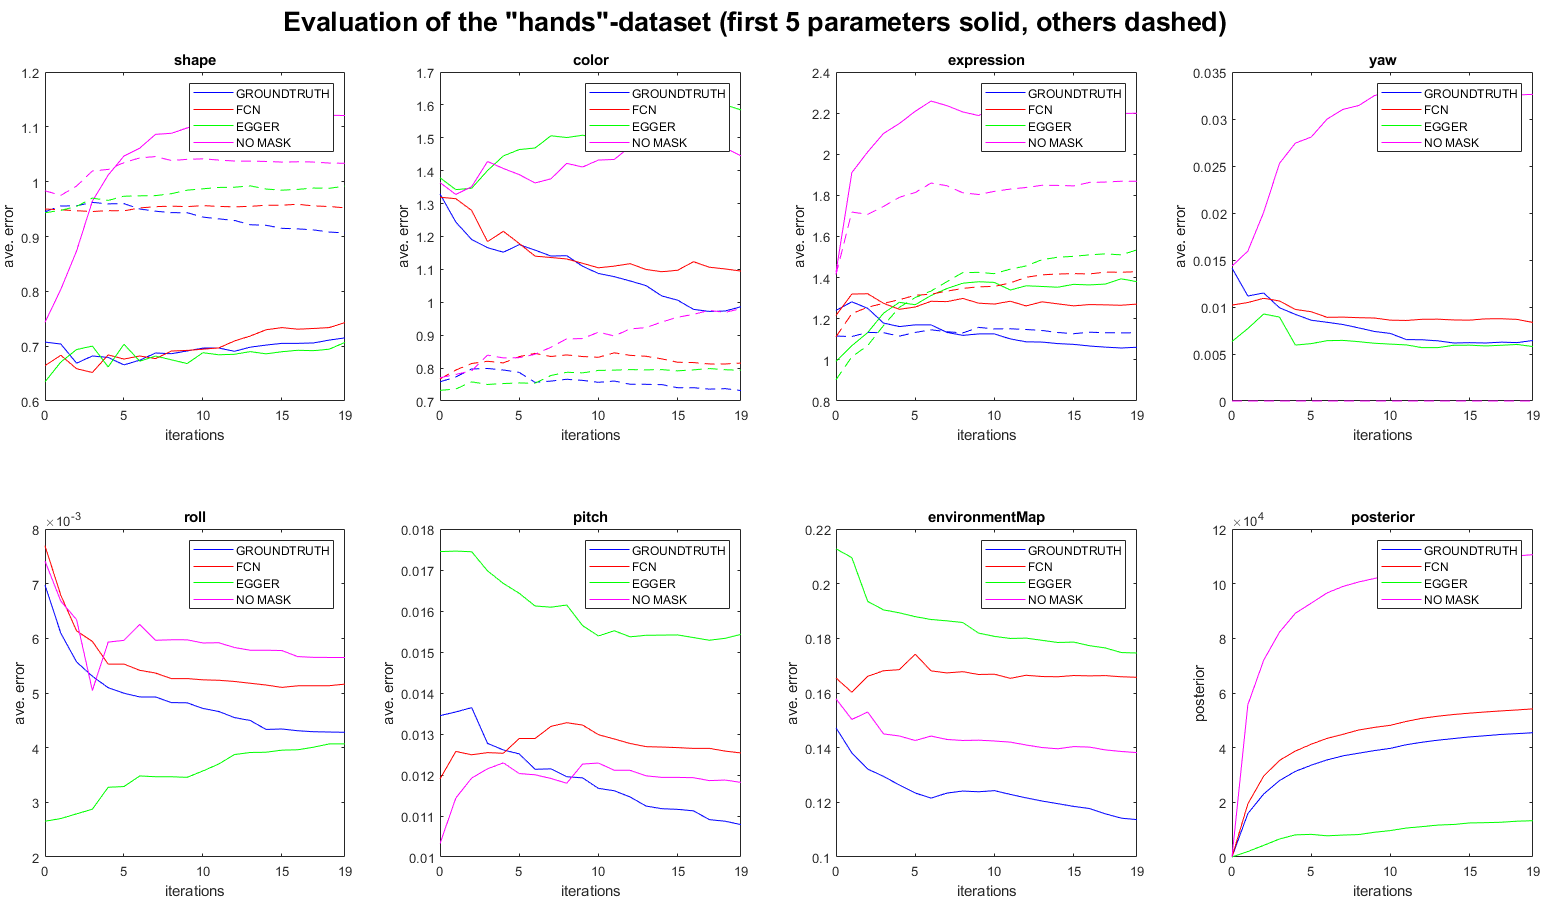
\includegraphics[angle=90,width=.55\textheight]{Figures/chap3/plot_hands_setting2.png}
	\caption{Due to the oversegmentation by Egger, a clear difference in the error of the color parameters can be seen. The mask of the FCN models the color significantly better.}
	\label{fig:chap3:plot_hands_setup2}
\end{figure}

\FloatBarrier

From these plots, we see that the method of Egger et al oversegments the synthetic face and segments regions which are not visible on the final fits (the 'face12' version of the Basel Face Model is used for fitting). Since these regions are also evaluated and have a slightly different colour from the rest of the face, the final colour is wrong. This is easy to see in the error-plots for the colour parameter (second plot) where the spread between the fit with the FCN mask and the one with the Egger mask is approximately 0.5 standard deviations.

\section{Runtime}

\begin{figure}[H]
	\begin{center}
		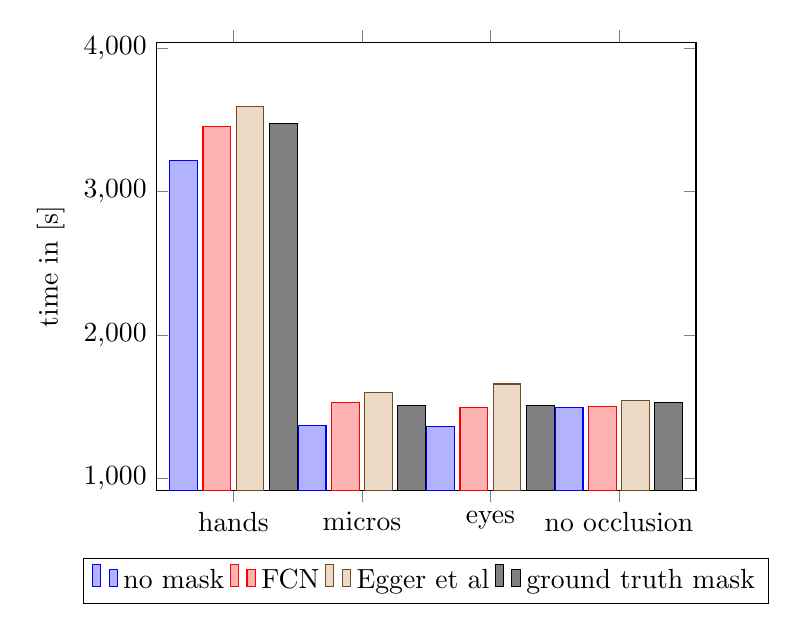
\begin{tikzpicture} 
		\begin{axis}[ 
		ybar, 
		enlargelimits=0.2, 
		legend style={at={(0.5,-0.15)}, anchor=north,legend columns=-1}, 
		ylabel={time in [s]}, 
		symbolic x coords={hands, micros, eyes, no occlusion}, 
		xtick=data, 
		%nodes near coords, 
		%nodes near coords align={vertical}, 
		] 
		
		\addplot coordinates {(hands,3220.89) (micros,1365.68) (eyes,1361.61) (no occlusion,1493.03)}; 
		\addplot coordinates {(hands,3457.30) (micros,1529.80) (eyes,1491.20) (no occlusion,1499.37)};
		\addplot coordinates {(hands,3597.28) (micros,1596.89) (eyes,1658.00) (no occlusion,1544.78)};
		\addplot coordinates {(hands,3476.42) (micros,1506.72) (eyes,1507.20) (no occlusion,1530.41)};
	
		
		\legend{no mask, FCN, Egger et al, ground truth mask} 
		\end{axis} 
		\end{tikzpicture}
	\end{center}
	\caption{Comparison of the Wall-Clock Time for the fitting process. The times were measured with the tailored 'face12' mask and the 'bfm' rendering.}
	\label{fig:chap3:times}
\end{figure}

Since we evaluated our experiments on a compute-server where we had no control of the priority of the process, we can't make a general statement about the absolute duration. Within a dataset, all fits for the different segmentations were computed simultaneously. From this, we can conclude that the fit with the FCN mask tends to require less time especially if the face is occluded by objects which can be recognised by the FCN.\\
\\
However, it is very difficult to make a general statement about the runtime behavior, because we cannot control whether the algorithm writes results in the cache and just loads them when desired, or computes them. As already mentioned, the Metropolis-Hastings algorithm proposes a randomly chosen sample to be the next one. If the evaluator rejects it, the algorithm uses the old sample as the next one and just has to load it from the cache.  